\newpage
	\section{Аффинная плоскость}
	\subsection{ГЛ1 1}
		А)\\
		Пусть точки трапеции $A, B, C, D$, где $AD \parallel BD$. Рассмотрим базис, начало которого $A$, базис-векторы $AB$ и $AD$.\\ 
		Тогда точки имеют координаты 
		\begin{gather*}
		A = (0,0)\\
		B = (1,0)\\
		C = (1,\alpha)\\
		D = (0,1)
		\end{gather*}
		Откуда\\
		AB: 
		\begin{gather*}
		\det 
		 \begin{pmatrix} 
				1 & x\\ 
				0 & y 
			\end{pmatrix} 
		= \det
			\begin{pmatrix} 
				1 & 0\\ 
				0 & 0 
			\end{pmatrix} 
		\Leftrightarrow x \cdot 0 + y \cdot 1 = 0
		\end{gather*}
		 
		CD:
		\begin{gather*}
		\det 
			\begin{pmatrix} 
				1 & x\\ 
				\alpha -1 & y 
			\end{pmatrix}
		= \det 
			\begin{pmatrix} 
				1 & 0\\ 
				\alpha -1 & 1 
			\end{pmatrix}\\
		\Leftrightarrow y - x \cdot \alpha + x = 1\\
		\Leftrightarrow x \cdot (1-\alpha) + y \cdot 1 = 0
		\end{gather*}
		 
		\begin{gather*}
		AB \cap CD: x \cdot 0 + y \cdot 1 = 0\\
		\Rightarrow x = \frac{1}{\alpha - 1} \quad y = 0\\
		x \cdot (1-\alpha) + y \cdot 1 = 0\\
		\Rightarrow
		\end{gather*}
		 
		AC:
		\begin{gather*}
		\det 
			\begin{pmatrix}
				1 & x\\
				\alpha & y 
			\end{pmatrix} 
		= \det 
			\begin{pmatrix} 
				1 & 0\\
				\alpha & 0 
			\end{pmatrix}
		\Leftrightarrow x \cdot (-\alpha) + y \cdot 1 = 0
		\end{gather*}
		 
		BD: 
		\begin{gather*}
		\det 
			\begin{pmatrix} 
				1 & x\\ 
				-1 & y 
			\end{pmatrix} 
		= \det 
			 \begin{pmatrix} 
				 1 & 0\\
				 -1 & 1 
			 \end{pmatrix}
		 \Leftrightarrow x \cdot 1 + y \cdot 1 = 1
		 \end{gather*}
		 
		 \begin{gather*}
		 AC\cap BD: x \cdot (-\alpha) + y \cdot 1 = 0\\
		 \Rightarrow 
		 \quad x = \frac{1}{\alpha + 1} 
		 \quad y = \frac{\alpha}{\alpha + 1}\\
		\\
		 x \cdot 1 + y \cdot 1 = 1 \Rightarrow\\
		 	M_1: (0;\frac{1}{2})\\
		 	M_2: (1;\frac{\alpha}{2})\\
		 	M_1M_2:\\ 	
		 	\det \begin{pmatrix} 1 & x\\ \frac{\alpha-1}{2} & y \end{pmatrix} = 
		 	\det \begin{pmatrix} 1 & 0\\ \frac{\alpha-1}{2} & \frac{1}{2} \end{pmatrix} 
		 	\quad \Leftrightarrow 
		 	\quad x \cdot (\frac{1-\alpha}{2}) + y = \frac{1}{2} 
		 	\end{gather*}
		 	
		 Заметим что $AB\cap CD$ и $AC\cap BD$ принадлежат этой прямой 
		 \begin{gather*}
		 \frac{1}{\alpha - 1} \cdot \frac{1-\alpha}{2} + 0 = \frac{1}{2} \quad
		 \frac{1}{\alpha + 1} \cdot \frac{1-\alpha}{2} + \frac{\alpha}{\alpha + 1} = \frac{1}{2}
		 \end{gather*}
		
		Б)\\		
		Пусть дан четырёхугольник $ABCD$, середины $AC$ и $BD$ - $M_1$ и $M_2$ соотв. Рассмотрим базис, центр которого $A$, базисные вектора $AB$ и $AD$. Тогда координаты точек\\
		\begin{gather*}
		A: (0;0),\\
		B : (1;0),\\
		C : (\alpha;\beta)\\
		D : (0;1)\\
		M_1 : (\frac{\alpha}{2};\frac{\beta}{2})\\ 
		M_2 : (\frac{1}{2};\frac{1}{2}) 
		\end{gather*}
		Далее прямые -\\ 
		\begin{gather*}
		AB:\\
		\det
		\begin{pmatrix}
			1 & x\\ 
			0 & y
		\end{pmatrix}
		 = \det 
		\begin{pmatrix}
			1 & 0\\ 
			0 & 0
		\end{pmatrix}
		\Leftrightarrow x \cdot 0 + y \cdot 1 = 0 		
		\end{gather*}
		 
		\begin{gather*}
		CD:\\
		\det
		\begin{pmatrix}
			\alpha & x\\ 
			\beta - 1 & y
		\end{pmatrix}
		= \det
		\begin{pmatrix}
			\alpha & 0\\ 
			\beta - 1 & 1
		\end{pmatrix}
		\Leftrightarrow -x \cdot (\beta - 1) + y \cdot \alpha = \alpha 
		\end{gather*}
		
		\begin{gather*}
		AB \cap CD:
			\begin{cases}
				x \cdot 0 + y \cdot 1 = 0\\ 
				-x \cdot (\beta - 1) + y \cdot \alpha = \alpha 
			\end{cases}
			\Leftrightarrow y = 0; x = -\frac{\alpha}{\beta - 1} 
		\end{gather*}
		
		Аналогично
		\begin{gather*}
		AD:\\
		\det
		\begin{pmatrix}
			0 & x\\ 
			1 & y
		\end{pmatrix}
		= \det
		\begin{pmatrix}
			0 & 0\\ 
			1 & 0
		\end{pmatrix}
		\Leftrightarrow x \cdot (-1) + y \cdot 0 = 0 
		\end{gather*}
		 
		\begin{gather*}
		BC:
		\det
		\begin{pmatrix}
			\alpha - 1 & x\\ 
			\beta & y
		\end{pmatrix}
		= \det
		\begin{pmatrix}
			\alpha - 1 & 0\\ 
			\beta & 0
		\end{pmatrix}
		\Leftrightarrow -x \cdot (\beta) + y \cdot (\alpha - 1) = -\beta 
		\end{gather*}
		
		\begin{gather*}
		AD\cap BC:
			\begin{cases}
			-x \cdot 1 + y \cdot 0 = 0\\ 
			-x \cdot \beta + y \cdot (\alpha - 1) = -\beta 
			\end{cases}
		\Leftrightarrow y = -\frac{\beta}{\alpha-1} \quad x = 0 
		\end{gather*}
		
		Таким образом середина $AB\cap CD$ и $AC\cap BD$, точка M имеет координаты\\
		$M$:
		$(-\frac{\alpha}{2 \cdot (\beta - 1)}; -\frac{\beta}{2 \cdot (\alpha - 1)}) $\\
		
		Покажем что $M_1$, $M_2$ и $M$ лежат на одной прямой .\\ 
		$M_1 M_2$ :
		\begin{gather*} 
		\det
		\begin{pmatrix}
			\frac{\alpha - 1}{2} & x\\ 
			\frac{\beta - 1}{2} & y
		\end{pmatrix}
		= \det
		\begin{pmatrix}
			\frac{\alpha - 1}{2} & \frac{1}{2}\\ 
			\frac{\beta - 1}{2} & \frac{1}{2}
		\end{pmatrix}		
		\Leftrightarrow
		-x \cdot \frac{\beta - 1}{2} + y \cdot \frac{\alpha - 1}{2} = \frac{\alpha - 1}{4} - \frac{\beta - 1}{4} 
		\end{gather*}
		
		Подставив в это выражение координаты точки $M$ получим 
		\begin{gather*} 
		-(-\frac{\alpha}{2 \cdot (\beta - 1)}) \cdot \frac{\beta - 1}{2} + (-\frac{\beta}{2 \cdot (\alpha - 1)}) \cdot \frac{\alpha - 1}{2} = \frac{\alpha - 1}{4} - \frac{\beta - 1}{4} 
		\end{gather*}


	\subsection{ГЛ1 2}
		Предположим $q$ составное, то есть существует такие $a$ и $b$, что $a,b \: \ne 0$ и $ab = q$. Тогда для точек $(0,0)$ и $(0,a)$ верно, что через них проходят 2 прямые,
		а именно с векторами (0,1) и $(b, 1)$, при этом очевидно, что эти прямые не совпадают. Из этого следует, что при составном $q$, $F_q$ не является аффинной плоскостью, поэтому $q$ простое.
		Заметим, что каждая прямая содержит ровно $q$ точек, так как каждой прямой можно сопоставить вектор $\overrightarrow{v}$, который в ней содержится и рассмотреть точки $a_1, a_2 , ... , a_q$, где $a_1$ - случайная точка на прямой, остальные $a$ задаются рекуррентно: $a_x = a_{x-1} + \overrightarrow{v}$. Очевидно, что $a_1 = a_{q + 1}$, так как $\overrightarrow{v}q = (0,0)$, при этом если есть точка $b$, принадлежащая прямой и не являющаяся одной из $a_1, a_2 , ... , a_q$, то $\overrightarrow{v}$ пропорционален $b - a_1$ $\Rightarrow$ $\overrightarrow{v}k_1 + (b - a_1) \cdot k_2 = 0$ $\Rightarrow$ $\overrightarrow{v}\frac{-k_1}{k_2} = (b - a_1)$ , при этом $\frac{-k_1}{k_2}$ однозначно определена на $F_q$ при простом $q \Rightarrow b$ принадлежит множеству $a_n$ $\Rightarrow$ на каждой прямой $q$ точек $\Rightarrow$ всего прямых = $\frac{q^2(q^2 - 1)}{q(q-1)} = q \cdot (q + 1)$ 
 
	\subsection{ГЛ1 3}
		Обозначим через $z_1$ , $z_2$ , ... , $z_m$ вершины ломаной, где $s_1$ лежит между $z_1$ и $z_2$, ... , $s_m$ лежит между $z_m$ и $z_1$.\\ 
		Заметим, что
		\begin{gather*}
		x_n = 2 \cdot s_n - x_{n-1}
		\end{gather*}
		Где $x_i = \overrightarrow{x_i x_0}$, $s_i = \overrightarrow{s_i x_0}$, $z_i = \overrightarrow{z_i x_0}$\\
		Откуда
		\begin{gather*}
		x_m = 2 \cdot s_m - x_{m-1}\\
		x_m = 2 \cdot s_m - (2 \cdot s_{m-1} - x_{m-2}) = 2 \cdot (s_m - s_{m-1}) + x_{m-2}\\
		...\\
		x_m = 2 \cdot (s_m - s_{m-1} + , ... , + s_1) - x_0
		\end{gather*}
		Заметим, что $s_i = \frac{z_i + z_{i + 1}}{2}$ ($i$ рассматривается по$\mod m$) из чего получаем, что
		\begin{gather*}
		2 \cdot (s_m - s_{m-1} + , ... , + s_1) - x_0 =\\
		(z_1 + z_m) - (z_m + z_{m-1}) + (z_{m-1} + z_{m-2}) - , ... , + (z_2 + z_1) - x_0 =\\
		z_1 \cdot 2 - x_0 = x_m
		\end{gather*}
		Из чего очевидно, что середина $x_0x_m$, т.е. $z_1$ является вершиной ломаной.\\
		
	\subsection{ГЛ1 4}
		Да, так как барицентр каждой из групп точек $P$ и $Q$ (точки $p_i$ и $q_j$) обладает свойством		 
		\begin{gather*}
		\sum_{i} \overrightarrow{c_p p_i} \cdot \mu_i = 0\\
		\sum_{j} \overrightarrow{c_q q_j} \cdot v_j = 0
		\end{gather*}		 
		 В то время как барицентр $c_p$ и $c_q$ с весами $\sum \mu_i = P$ и $\sum v_j = Q$ соответственно, причем $|P|, |Q| > 0$. Пусть $c$ - такая точка, что
		 \begin{gather*}
		 \overrightarrow{c c_p} \cdot P + \overrightarrow{c c_q} \cdot Q = 0
		 \end{gather*}		 
		 При этом для каждого $p_i$ верно, что 
		 \begin{gather*}
		 \overrightarrow{c c_p} + \overrightarrow{c_p p_i} = \overrightarrow{c p_i}
		 \end{gather*}		 
		 Из чего следует, что сложив выражения $\sum_{i} \overrightarrow{c_p p_i} \cdot \mu_i = 0$, $\sum_{j} \overrightarrow{c_q q_j} \cdot v_j = 0$ и $\overrightarrow{c c_p} \cdot P + \overrightarrow{c c_q} \cdot Q = 0$, получается
		 \begin{gather*}
		 \biggl(\sum_{i} \overrightarrow{c_p p_i} \cdot \mu_i + \overrightarrow{c c_p} \cdot P \biggl) + \biggl( \sum_{j} \overrightarrow{c_q q_j} \cdot v_j + \overrightarrow{c c_q} \cdot Q \biggl) = 0
		 \end{gather*}		 
		 Что равносильно
		 \begin{gather*}
		 \sum_{i} \overrightarrow{c p_i} \cdot \mu_i + \sum_{j} \overrightarrow{c q_j} \cdot v_j = 0
		 \end{gather*}		 
		 Из чего следует то, что $c$ является барицентром всей системы.
				
\newpage
		 \subsection{ГЛ1 5}
		 Докажем, что возможность расставить массы $\alpha$, $\beta$ и $\gamma$ равносильна тому, что $a_1$, $b_1$ и $c_1$ являются основаниями чевиан.\\
		 \\
		 1. (Массы $\Rightarrow$ Чевианы) \\
		 Возможность расставить массы означает, что центр масс находится на прямых $a a_1$, $b b_1$ и $c c_1$, из чего следует пересечение этих прямых в одной точке.\\
		 \\	 
		 2. (Чевианы $\Rightarrow$ Массы) \\
		 Если прямые пересекаются в одной точке, то точку пересечения можно выбрать как центр масс.\\
		 \\		 
		 1)\\
		 Теперь заметим, что если можно расставить массы, то можно рассмотреть отношение, в котором барицентры сторон делят стороны:
		 \begin{gather*}
		 \alpha_b : \alpha_c = \beta : \gamma\\
		 \beta_c : \beta_a = \gamma : \alpha\\
		 \gamma_a : \gamma_b = \alpha : \beta
		 \end{gather*}
		 И тогда $\frac{\alpha_b \cdot \beta_c \cdot \gamma_a}{\alpha_c \cdot \beta_a \cdot \gamma_b} = \frac{\beta \cdot \gamma \cdot \alpha}{\gamma \cdot \alpha \cdot \beta} = 1$\\
		 Т.е. $aa_1,\: bb_1,\: cc_1$ это чевианы
		 \\
		 2)\\
		 В свою очередь, если равенство$\biggl( \frac{\alpha_b \cdot \beta_c \cdot \gamma_a}{\alpha_c \cdot \beta_a \cdot \gamma_b} = 1 \biggl)$ верно, то можно расставить массы
		 $\gamma_a$, $\gamma_b$ и $\frac{\alpha_b \cdot \gamma_a}{\alpha_c}$ так, что:\\
		 $c_1$ является барицентром $A$ и $B$ ($\gamma_a : \gamma_b \: = \: \gamma_a : \gamma_b$);\\
		 $a_1$ является барицентром $B$ и $C$ ($\frac{\alpha_b \cdot \gamma_a}{\alpha_c} : \gamma_a = \alpha_b : \alpha_c$);\\
		 $b_1$ является барицентром $A$ и $C$ ($\frac{\alpha_b \cdot \gamma_a}{\alpha_c} : \gamma_b = \beta_a : \beta_c)$;\\
	\subsection{ГЛ1 6}
		 		
		 Заметим, что барицентрические координаты точек\\
		 \begin{tabbing}
		 	$a_1$\= (\=-$|\overrightarrow{b_1 c}|$ \= ;\= -$|\overrightarrow{a_1 c}|$\=;\=-$|\overrightarrow{a_1 b}|$\=) \kill
		 	$a_1$\> (\>0\>;\> -|$\overrightarrow{a_1 c}$|\>;\> |$\overrightarrow{a_1 b}$| \>)\\
		 	$b_1$\> (\>|$\overrightarrow{b_1 c}$| \> ;\>0\>;\> -|$\overrightarrow{b_1 a}$| \>)\\
		 	$c_1$\> (\> -|$\overrightarrow{c_1 b}$| \> ;\> |$\overrightarrow{c_1 a}$| \>;\>0\>)\\
		\end{tabbing}	 	
		Заметим, что если $a_1 b_1 c_1$ - прямая $\Leftrightarrow$ 
		\\$c_1$ представимо в виде линейной комбинации точек $a_1$ и $b_1$ $\Leftrightarrow$ 
		\begin{gather*}
		x_1 \cdot a_1 + x_2 \cdot b_1 = c_1 \Leftrightarrow\\
		\overrightarrow{b_1 c} \cdot x_2 = -\overrightarrow{c_1 b}\Leftrightarrow\\\\
		x_2 = -\frac{\overrightarrow{c_1 b} }{\overrightarrow{b_1 c} } 
		\overrightarrow{c_1 a} = -\overrightarrow{a_1 c} \cdot x_1 \Leftrightarrow\\\\
		x_1 = -\frac{\overrightarrow{c_1 a} }{\overrightarrow{a_1 c} }
		\overrightarrow{a_1 b} \cdot x_1 - \overrightarrow{b_1 a} \cdot x_2 = 0 \Leftrightarrow\\\\
		\overrightarrow{a_1 b} \cdot x_1 = \overrightarrow{b_1 a} \cdot x_2 \Leftrightarrow\\\\
		\overrightarrow{a_1 b} \cdot \overrightarrow{c_1 a} \cdot \overrightarrow{b_1 c} = \overrightarrow{a_1 c} \cdot \overrightarrow{c_1 b} \cdot \overrightarrow{b_1 a} \Leftrightarrow\\\\
		(\overrightarrow{a_1 b}:\overrightarrow{a_1 c}) \cdot (\overrightarrow{c_1 a}:\overrightarrow{c_1 b}) \cdot (\overrightarrow{b_1 c}:\overrightarrow{b_1 a}) = 1
		\end{gather*} 
		что и требовалось доказать 

	\subsection{ГЛ1 7}
		A)\\
		Заметим, что если один четырёхугольник перешёл в другой, то отношение отрезков на диагоналях сохраняется, образ пересечения диагоналей это пересечение диагоналей образного четырёхугольника. При этом, если 2 четырёхугольника $ABCD$ и $EFGH$ имеют одинаковое отношение отрезков на диагоналях $(\frac{AO}{AC} = \frac{EU}{EG} = \alpha; \: \frac{BO}{BD} = \frac{FU}{FH} = \beta)$, то можно перевести один в другой аффинным преобразованием, а именно переведя треугольник $ABC$ в $EFG$, тогда $O$ будет иметь барицентрические координаты ($\alpha; \: 1; \: 1 - \alpha$) относительно $ABC$. Такие же координаты имеет и точка U, относительно $EFG$. Аналогично D: ($\alpha \cdot (1 - \beta); \: 1; \: (1 - \alpha) \cdot (1 - \beta)$) (c точностью до домножения на константу), имеет такие же кординаты, что и $H$ относительно $EFG$.\\
		Ответ: да\\
		\\
		Б)\\
		Заметим, что отношения отрезков диагоналей равны отношению оснований трапеции $ABCD$ ($BC \parallel AD$), так как рассмотрим репер $(A, \overrightarrow{AC}, \overrightarrow{AD})$, тогда точка $B$ - $(1; -\alpha)$, $D$ - $(0;1)$. Заметим, что $O$ имеет координаты $(\frac{1}{1 + \alpha};0)$, так как $\overrightarrow{v} = (1; - 1 - \alpha)$, $BOD$ лежат на одной прямой $\: \Leftrightarrow \: \det(O, \overrightarrow{v}) = \det((0;1), \overrightarrow{v}) \: \Leftrightarrow \: \frac{1}{1 + \alpha} \cdot (-1) \cdot (1 + \alpha) = -(1) \cdot (1) \: \Leftrightarrow \: -1 = -1$. Откуда следует, что ответ такой же, что и в (7A).\\
		Ответ: да\\
		\\
		
		\subsection{ГЛ1 8}
		
		\subsection{ГЛ1 9}
		Впишем правильный многоугольник в окружность радиуса $r = 1$, тогда все векторы $|v_1| = |v_2| = ... = |v_n| = 1$ и, если $S_1$ - площадь правильного многоугольника, то $S_1 < \pi r^2 = \pi 1^2 = \pi$. Обозначим $S_2 = \det(v_1, v_2) + \det(v_2, v_3) + ... + \det(v_n, v_1)$, тогда если $S_2 > 2\pi$, то $S_2 > 2S_1$. Приведем пример такого n-угольника, для которого это выполнено
		
		\begin{figure}[h]
			\center{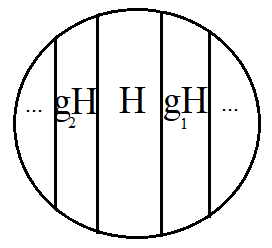
\includegraphics[width=1.0\linewidth]{Pic1}}
		\end{figure}	
		\newpage
		Рассмотрим 20-угольник, разобьем его вершины на 5 групп по 4 вершины, причем в каждую группу входят вершины, идущие через 5. И занумерыем вершины так: 
		$A_{1}$, $A_{5}$, $A_{9}$, $A_{13}$, $A_{17}$, $A_{2}$, $A_{6}$, $A_{10}$, $A_{14}$, $A_{18}$, $A_{3}$, $A_{7}$, $A_{11}$, $A_{15}$, $A_{19}$, $A_{4}$, $A_{8}$, $A_{12}$, $A_{16}$, $A_{20}$.\\
		Тогда каждая из групп будет образовывать квадрат со стороной $\sqrt{2}$, а все остальные треугольники будут положительной площади, так как если мы рассмотрим 2 подряд идущие точки из разных групп, то их площадь будет положительна, так как направленный угол, образованый этими 2 векторами будет $< 180^o$, так как они идут через 6 других точек, а в одной полуплоскости находятся 10 точек $\Rightarrow$ $S_2 > 5 \cdot (\sqrt{2})^2 > 2 \pi > 2S_1$, что и требовалось.